\title{Loom: High performance blockchain }

\author{
        Anatoly Yakovenko \\
        aeyakovenko@gmail.com\\
}
\date{}

\documentclass[12pt]{article}

\usepackage{graphicx}

\begin{document}
\maketitle

\begin{abstract}
A new Proof of History algorithm is proposed for global read consistency which can be used alongside a consensus algorithm to minimize messaging overhead in a Byzantine Fault Tolerant replicated state machine. It achieves performance by creating a single globally agreed upon order of events independent of network consensus. Nodes participating in the network only vote on a binary choice of accepting or rejecting the ordering. Without hardware failures, all the participating nodes are expected to agree with the proposed ordering with minimal communication overhead above the transaction data itself. Any consensus algorithm can be used, such as Proof of Work or Proof of Stake, a simple Proof of Stake consensus algorithm is proposed. To ensure high availability of data, an efficient streaming Proof of Replication is proposed which takes advantage of the time keeping properties provided by Proof of History.  The combination of PoRep and PoH provides a substantial defense against forgery of the ledger in terms of time and storage. The protocol is analyzed on a 1gbps network, and it is shown that throughput is limited by network or ECDSA digests, and with a GPU dedicated to ECDSA digests over \textbf{350k} and up to \textbf{700k} transactions per second with high availability is theoretically possible.

\end{abstract}

\section{Introduction}
This is time for all good men to come to the aid of their party!

%\paragraph{Outline}
%The remainder of this article is organized as follows.
%Section~\ref{previous work} gives account of previous work.
%Our new and exciting results are described in Section~\ref{results}.
%Finally, Section~\ref{conclusions} gives the conclusions.

\section{Design}\label{design}

Loom is a Proof of History generator.  It takes a sequence of arbitrary user transactions.  It orders them in the most efficient way to process them, by maximizing memory throughput.  Executes the transactions on the current state that is stored in RAM.  Publishes the transactions and a signature of the state stored in RAM to the replications nodes.  Spools replicate the operations on their copies of the state, and publish their computed hash as confirmations via consensus algorithm.

\begin{figure}
  \begin{center}
    \centering
    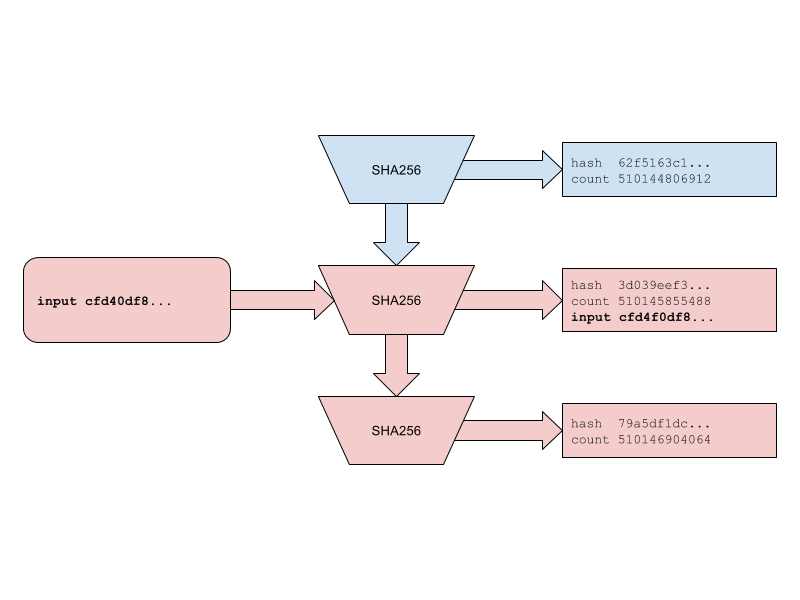
\includegraphics[width=0.9\textwidth]{figures/fig_1.png}
    \caption[Fig 1]{Transaction flow throught the network.\label{fig_1}}
  \end{center}
  \end{figure}

In the figure above, messages are sent by users into the Loom node, which orders them and broadcasts the order and the resulted computed state to the replicator nodes called Spools.  Spools then send a confirmation message of the computed state hash to the Loom.

Looms are elected by the network via its configured consensus algorithm, such as Proof of Stake or Proof of Work.  More on elections here.

Proof of History sequence guarantees global read consistency for the network that would require an attacker an investment of time to reverse.  A Proof of Stake algorithm is proposed for electing Looms and posting confirmations of the order.  A fast Proof of Replication is proposed for ledger and state availability, and as a defense against forgery attacks.

\section{Proof of History}\label{proof_of_history}

Proof of History provides a way to cryptographically verify passage of time between two events. It uses a cryptographically secure function whose output cannot be predicted from the input, and must be completely executed to generate the output. The function is run in a sequence, it’s previous output as the current input, periodically recording the current output, and how many times it’s been called. The output can then be recomputed and verified by external computers in parallel by checking each period in parallel on a separate core. Data can be timestamped into this sequence by recording the data and the index it was mixed into the sequence. The timestamp then guarantees that the data was created sometime before this hash was generated in the sequence. Multiple generators can synchronize amongst each other by mixing their state into each others sequences. \\

\subsection{Description}

With a cryptographic function, like a cryptographic hash (sha256, md5,
sha-1), whose output cannot be predicted without running the function,
run the function from some random starting value and take its output
and pass it as the input into the same function again. And record the
number of times the function has been called and the output at each
call. \\\\
\noindent For example: \\\\\noindent
\texttt{
  sha256(\char`\"any random starting value\char`\") $\rightarrow$
  hash1, (n\_count~$=~1$) \\
  sha256(hash1) $\rightarrow$ hash2, (n\_count~$=~2$)\\
  sha256(hash2) $\rightarrow$ hash3, (n\_count~$=~3$)\\
}

\noindent Where \texttt{hashN} represents the actual hash output. \\

Instead of publishing every hash on every index, only a subset of
these hashes could be published at an interval.\\

\noindent For example:\\\\\noindent
\texttt{
 sha256(\char`\"any starting value\char`\") $\rightarrow$ hash1, (n\_count~$=1$)\\
\ldots\\
sha256(hash199) $\rightarrow$ hash200, (n\_count~$=200$)\\
\ldots\\
sha256(hash299) $\rightarrow$ hash300, (n\_count~$=300$)\\
}

This set of events can only be computed in sequence by a single computer thread, because there is no way to predict what the hash value at index $300$ is going to be without actually running the algorithm from the starting value $300$ times.

\begin{figure}
  \begin{center}
    \centering
    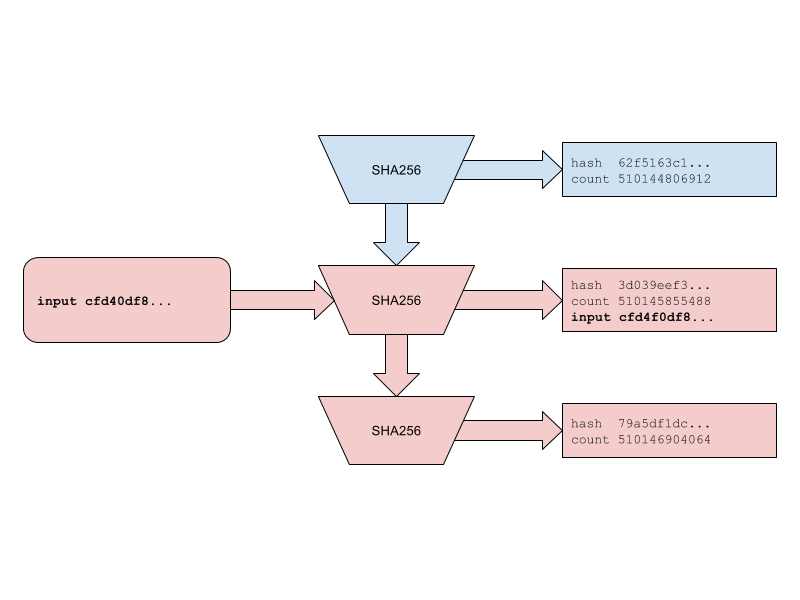
\includegraphics[width=0.6\textwidth]{figures/fig_2.png}
    \caption[Fig 2]{Figure description \label{fig_2}}
  \end{center}
  \end{figure}
%A much longer \LaTeXe{} example was written by Gil~\cite{Gil:02}.
In the example in Figure 1, hash \texttt{62f51643c1} was produced on
count $510144806912$ and hash \texttt{c43d862d88} was produced on
count $510146904064$. Real time passed between count $510144806912$
and count $510146904064$.

\subsection{Timestamp for Events}

This sequence of hashes can also be used to record that some piece of data was created before a particular hash index was generated.  Using a `combine` function to combine the piece of data with the current hash at the current index. The `data` can simply be a cryptographically unique hash of arbitrary event data. The combine function can be a simple append of data, or any operation that is collision resistant.\\

Arithmetic operations like addition, multiplication etc... wouldn’t work because an attacker could have precomputed a separate sequence in parallel, and could join the two by inserting a piece of data that would add up to the starting value of the parallel sequence. Append would force the attacker to try to create a collision between a hash, and the data they are trying to append.\\


\noindent For example:\\\\\noindent
\texttt{
sha256(\char`\"any starting value\char`\") $\rightarrow$ hash1,
(n\_count $=~1$)1\\
\ldots\\
sha256(hash199) $\rightarrow$ hash200, (n\_count $=~200$)\\
\ldots\\
sha256(hash299) $\rightarrow$ hash300, (n\_count $=~300$)\\
}

\noindent Some external event occurs, like a photograph was taken, or
any arbitrary digital data was created:\\\\\noindent
\texttt{
  sha256(hash334) $\rightarrow$ hash335, (n\_count $=~335$), photograph\_sha256\\
  sha256(append(hash335, photograph\_sha256) $\rightarrow$ hash336,
  (n\_count $=~336$)\\
  \ldots\\
  sha256(hash399) $\rightarrow$ hash400, (n\_count $=~400$)\\
}

\texttt{Hash336} is computed from the appended binary data of
\texttt{hash335} and the \texttt{sha256} of the photograph. The index,
and the \texttt{sha256} of the photograph are recorded as part of the
sequence output. So anyone verifying this sequence can then recreate
this change to the sequence. The verifying can still be done in
parallel:\\\\\noindent
\texttt{
  sha256(hash299) $\rightarrow$ hash300, (n\_count $=~300$)\\
  sha256(hash334) $\rightarrow$ hash335, (n\_count $=~335$), photograph\_sha256\\
}\\\noindent
And\\\\\noindent
\texttt{
  sha256(append(hash335, photograph\_sha256) $\rightarrow$ hash336,
  (n\_count $=~336$)\\
  sha256(hash399) $\rightarrow$ hash400, (n\_count $=~400$)\\
}

Because the initial process is still sequential, we can then tell that things entered into the sequence must have occurred sometime before the future hashed value was computed.\\\\\noindent
\texttt{
sha256(hash334) $\rightarrow$ hash335, (n\_count $=~335$), photograph1\_sha256\\
sha256(append(hash335, photograph\_sha256) $\rightarrow$ hash336,
(n\_count $=~336$)\\
\ldots\\
sha256(hash599) $\rightarrow$ hash600, (n\_count $=~600$), photograph2\_sha256
sha256(append(hash600, photograph2\_sha256) $\rightarrow$ hash601,
(n\_count $=~601$)\\
}

So \texttt{photograph2} was created before \texttt{hash601}, and
\texttt{photograph1} was created before \texttt{hash336}. Inserting this extra data into the sequence of hashes results in an unpredictable change to all subsequent values in the sequence. So it would be impossible to precompute any future sequences based on prior knowledge of what data will be mixed into the sequence.\\

The sequence only needs to mix and publish a hash of the event data into the event sequence. The mapping of the hash to event data can be stored outside of the sequence, and the event data can contain other metadata within itself, such as real time stamps and connection IPs.\\

\begin{figure}
  \begin{center}
    \centering
    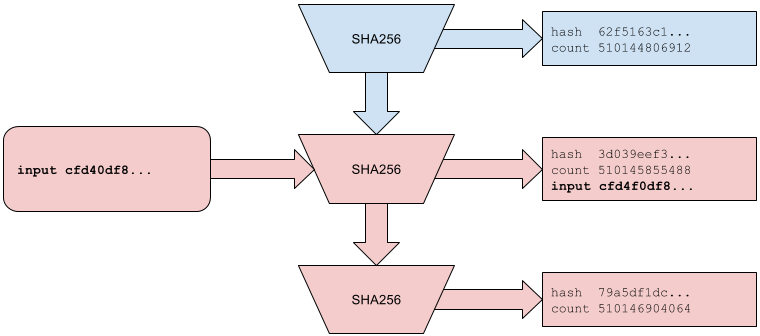
\includegraphics[width=0.9\textwidth]{figures/fig_3.png}
    \caption[Fig 3]{Figure description \label{fig_3}}
  \end{center}
  \end{figure}

  In the example in Figure 2, input \texttt{cfd40df8\ldots} was inserted into the Proof of History sequence. The count at which it was inserted is $510145855488$ and the state at which it was inserted it is \texttt{3d039eef3}.\\

Every node observing this sequence can determine the order at which all events have been inserted. Generating a reverse order would require an attacker to start the malicious sequence after the second event. This delay would allow any non malicious peer to peer nodes to communicate about the original order.\\

\subsection{Verification}
The sequence can be verified as correct in a multi core computer in less time than it took to generated it 

\noindent For example: \\\\\noindent

Core1:
sha256(\char`\"any random starting value\char`\") $\rightarrow$ hash1, 1
...
sha256(hash199) $\rightarrow$ hash200, 200

Core2:
sha256(hash199) $\rightarrow$ hash200, 200
...
sha256(hash299) $\rightarrow$ hash300, 300


So given some number of cores, like a modern GPU with 4000 cores, the verifier can split up the sequence of hashes and their indexes into 4000 slices, and in parallel make sure that each slice is correct from the starting hash to the last hash in the slice.  So if the expected time to produce the sequence is going to be 

<number of hashes>/<hashes per second for 1 core>

the expected time to verify that the sequence is correct is going to be 

<number of hashes>/(<hashes per second per core> * <number of cores available to verify>)

\begin{figure}
  \begin{center}
    \centering
    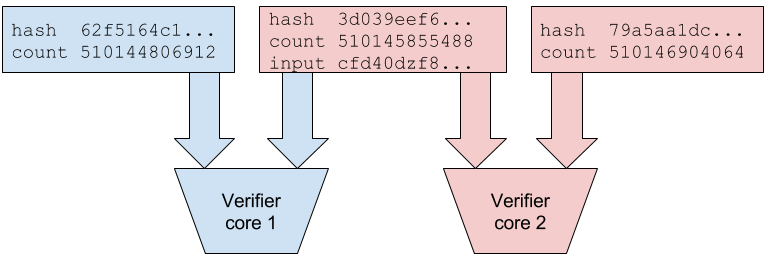
\includegraphics[width=0.9\textwidth]{figures/fig_4.png}
    \caption[Figure 4]{Verification using multiple cores\label{fig_4}}
  \end{center}
  \end{figure}

In the example in Figure 3, each core is able to verify each slice of the sequence in parallel.  Since all input strings are recorded into the output, with the counter and state that they are appended to, the verifiers can replicate each slice in parallel.

\subsection{Horizontal Scaling}
It’s possible to synchronize multiple Proof of History generators by mixing the sequence state from each generator to each other generator, and thus achieve horizontal scaling of the Proof of History generator.

Generator A
Hash1a
Hash2a
Hash3a hash(Hash2b, hash1a)
Hash4a

Generator B
Hash1b
Hash2b
Hash3b hash(Hash2a, hash1b)
Hash4b

GeneratorA receives a data packet from Generator B, which contains the last state from Generator B, and the last state generator b observed from GeneratorA.  The next state hash in Generator A then depends on the state from Generator B, so we can derive that hash2b happened sometime before hash4a.  This property can be transitive, so if three generators are synchronized through a single common generator A ⇔ B ⇔ C, we can trace the dependency between A and C even though they were not synchronized directly.

By periodically synchronizing the generators, each generator can then handle a portion of external traffic, thus the overall system can handle a larger amount of events to track at the cost of the accuracy due to network latencies between the generators.

Having multiple generators may make deployment more resistant to attacks.  One generator could be high bandwidth, and receive many events to mix into its sequence, another generator could be high speed low bandwidth that periodically mixes with the high bandwidth generator.

The high speed sequence would create a secondary sequence of data that an attacker would have to reverse.

\begin{figure}
  \begin{center}
    \centering
    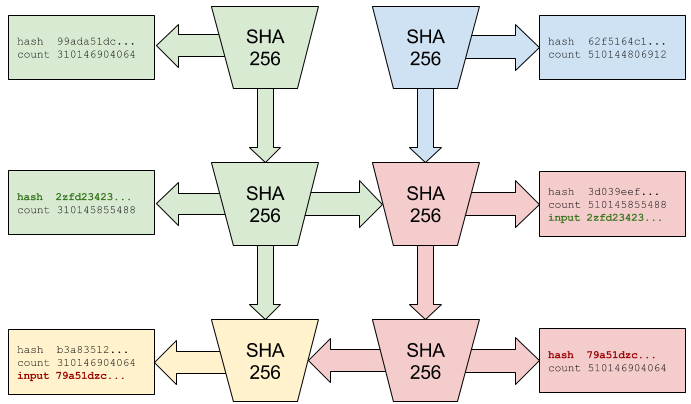
\includegraphics[width=0.9\textwidth]{figures/fig_5.png}
    \caption[Fig 5]{Two generators synchronizing\label{fig_5}}
  \end{center}
  \end{figure}

In the figure above, the two generators insert each other’s output state and record the operation.  

The synchronization is transitive.  A ⇔ B ⇔ C  There is a provable order of events between A and C through B.  Two generators can double bandwidth at the cost of availability.  10x1gbps connections with availability of 0.999 would have 0.999**10 -> 0.99 availability.
\subsection{Consistency}
Users can enforce consistency of the generated sequence and make it resilient to attacks by inserting the last observed output of the sequence they consider valid into their input.

hash9a
Event1, hash10a
Event2, hash20a
Event3, hash30a

If the events were all available to insert at the same time, or the service has a hidden clock that's slightly faster, the service could produce a second hidden sequence with the events in reverse order.  

hash9a
Event3, hash10b
Event2, hash20b
Event1, hash30b

Both sequences start at hash9a, so they are equal in length.  But as clients of this service, we want only a single valid sequence to exist. 

To prevent this attack, each client generated Event should contain within itself the latest hash that the client observed from what it considers to be a valid sequence.  So when a client creates the “Event1” hash, they should append the last hash they have observed.

Hash5a
Event1 = hash(append(event1 data, hash5a))
Event1, hash10a
hash15a
Event2 = hash(append(event2 data, hash15a))
Event2, hash20a
hash25a
Event3 = hash(append(event3 data, hash25a))
Event3, hash30a

When the sequence is published, Event3 would be referencing hash25a, and if it’s not in the sequence prior to this Event, the consumers of the sequence know that it’s an invalid sequence.  The partial reordering attack would then be limited to the number of hashes produced while the client has observed an event and when the event was entered.  Clients can then write software that doesn’t assume the order is correct for the short period of hashes between the last observed and inserted hash.

To prevent a malicious clock service from rewriting the client Event hashes, the clients can submit a signature of the event data and the last observed hash instead of just a hash

Event3 = sign(append(event3 data, hash25a), client Private Key)
Event3, hash30a

The mapping from the event hash or signature to event data and client’s public key can be published in a separate database for all the clients of the service to verify.
Verify:
	(Public Key, hash25a, event3 data) <- lookup Event3 
      Verify Event3 signature with Public Key
      Verify hash25a exists prior to hash31a in the sequence

\begin{figure}
  \begin{center}
    \centering
    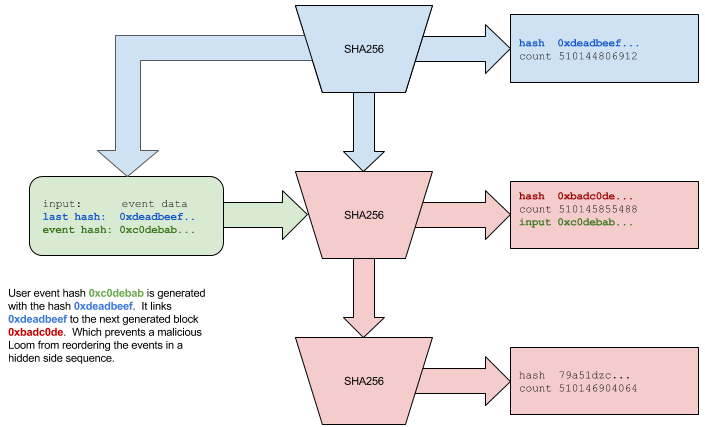
\includegraphics[width=0.6\textwidth]{figures/fig_6.png}
    \caption[Fig 6]{Input with a back reference.\label{fig_6}}
  \end{center}
  \end{figure}

The above example, user supplied input is dependent on hash 0xdeadbeef existing in the generated sequence sometime before it’s inserted.
\subsection{Advantages}

Proof of history provides some protection against long range attacks.  A malicious user that gains access to old private keys would have to recreate a historical record that takes as much time as the original one they are trying to forge.  This would require access to a faster processor than the network is currently using, otherwise the attacker would never catch up in history length.

Additionally, a single source of time allows for construction of a simper Proof of Replication (more on that later).  Since all the participants in the network can rely on a single historical record of events.  

PoRep and PoH together provide a defense of both space and time against a forged ledger.

\section{Proof of Stake Consensus}
\subsection{Description}
This specific instance of Proof of Stake is designed for quick confirmation of the current sequence produced by the Proof of History generator, for voting and selecting the next Proof of History generator, and for slashing any misbehaving validators.  This algorithm depends on messages eventually arriving to all participating nodes within a certain timeout.
\subsection{Bonding}
A bonding transaction takes a user specified amount of coin and moves it to a bonding account under the user’s identity.  Coins in the bonding account cannot be spent, and have to remain in the account until the user removes them.  The user can only remove stale coins that have timed out. 
\subsection{Voting}
Proof of History generator will publish a hash at a predefined period.  Each bonded identity must vote to approve the hash, and all the ordered transactions before it.  The vote is a simple Yes vote, without a no.

If 2/3rds of the bonded identities have voted within a timeout, that implies that either this history is valid, or a 1/3rd have voted duplicity.

\subsection{Unbonding}

Missing N number of votes marks the coins as stale and no longer eligible for voting.  The user can issue an unbonding transaction to remove them.
\subsection{Elections}
Election for a new PoH generator occur when the PoH generator failure is detected.  The validator with the largest voting power, or highest public key address if there is a tie is picked as the new PoH generator.

2/3rds of confirmations are required on the new sequence.  If the new leader fails before 2/3rds confirmations are available, the next highest validator is selected, and new set of conformations is required.

To switch votes, a validator needs to vote at a higher PoH sequence counter, and the new vote needs to contain the votes it wants to switch.  Otherwise the second vote will be slashable. Vote switching can only occur at a height that doesn’t have 2/3rds majority.

Once a PoH generator is established, a Secondary can be elected to take over the transactional processing duties.  If a Secondary exists, it will be considered as the next leader during a Primary failure.

Secondary and lower rank generators are promoted to Primary at a predefined schedule, or if an exception is detected.
\subsection{Election Triggers}
Forked Proof of History generator

PoH generators have an identity that signs the generated sequence.  A fork can only occur in case the PoH generator identity has been compromised.  A fork is detected because two different historical records have been published on the same PoH identity.

\subsubsection{Runtime Exceptions}
A hardware failure or a bug, or a intentional error in the PoH generator could cause it to generate an invalid state and publish a merkle of the state that doesn’t match the local validators result.  Validators will publish the correct merkle via gossip and this event would trigger a new round of elections.  Any validators who accept an invalid state will have their bonds slashed.

\subsubsection{Network Timeouts}

A network timeout would trigger an election.

\subsection{Slashing}
Slashing occurs when a validator votes duplicity for two separate sequences.  A proof of duplicit vote will remove the bonded coins from circulation and add them to the mining pool.

A vote that includes a previous vote on a contending sequence is not eligible as proof of duplicit voting.  If presented, it will remove the currently cast vote on the contending sequence.

Slashing also occurs if a vote is cast for an invalid hash generated by the PoH generator.  The generator is expected to randomly generate an invalid state which would trigger a fallback to Secondary.
Secondary Elections
Secondary and lower ranked Proof of History generators can be proposed and approved.  A proposal is cast on the primary generators sequence.  The proposal contains a timeout, if the motion is approved by 2/3rds of the vote before the timeout, the Secondary is considered elected, and will take over duties as scheduled.  Primary can do a soft handover to secondary by inserting a message into the generated sequence indicating that a handover will occur, or inserting an invalid state and forcing the network to fallback to Secondary.

If a Secondary is elected, and the primary fails, the secondary will be considered as the first fallback during an election.

\subsection{Attacks}
\subsubsection{Tragedy of Commons}

The PoS verifiers simply confirm the state hash generated by the PoH generator.  There is economic incentive for them to do no work and simply approve every generated state hash.  

To avoid this condition, the PoH generator should generate an invalid hash with a probability P.  Any voters for this hash should be slashed.  When the hash is generated, the network should immediately promote the Secondary elected PoH generator.

\subsubsection{Collusion with the PoH generator}
A verifier that is colluding with the PoH generator would know in advance when the invalid hash is going to be produced and not vote for it.  This scenario is really no different than the PoH identity having a larger verifier stake.  The PoH generator still has to do all the work to produce the state hash.
\section{Streaming Proof of Replication}
\subsection{Description}
Filecoin proposed a version of Proof of Replication (https://filecoin.io/proof-of-replication.pdf).  The goal of this version is to have fast and streaming verifications of Proof of Replication which are enabled by keeping track of time in Proof of History generated sequence.  Replication is not useful as a consensus algorithm, but is a useful tool to distribute the cost of storing the blockchain history or state at a high availability.
\subsection{Algorithm}
CBC encryption encrypts each block of data in sequence, using the previously encrypted block to XOR the input data.


Current block to be encrypted
Previous encrypted block data to be XORd with the current block before encryption
Ensures that the encryption can only be done sequentially, and it can be streamed

\begin{figure}
  \begin{center}
    \centering
    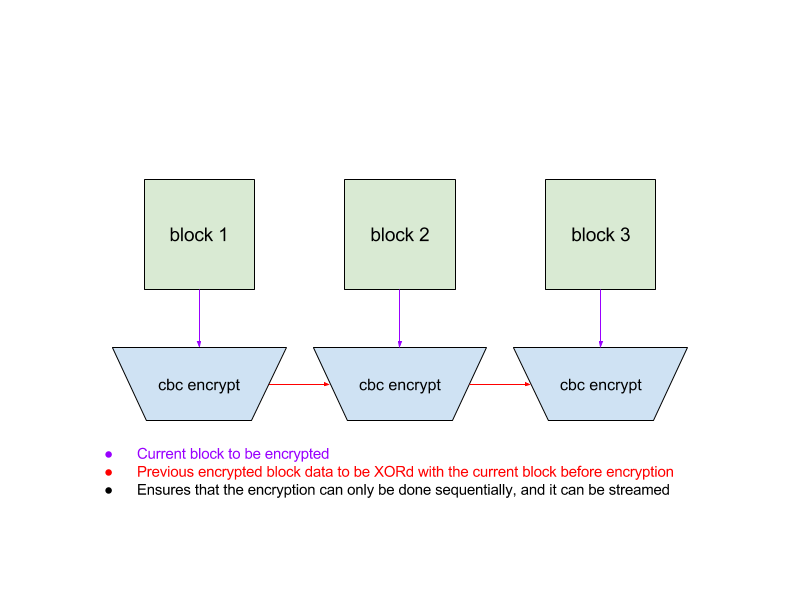
\includegraphics[width=0.6\textwidth]{figures/fig_7.png}
    \caption[Fig 7]{Figure description \label{fig_7}}
  \end{center}
  \end{figure}

Each replication identity generates a key by signing a hash that has been generated Proof of History sequence.  This ties the key to a replicators identity, and to a specific Proof of History sequence.  Only specific hashes can be selected.  (See Hash Selection)

The data set is fully encrypted block by block.  Then to generate a proof, the key is used to seed a pseudorandom number generator that selects a random 32 byte slice from each block.

A merkle hash is computed with the selected hash prepended to the each slice.

\begin{figure}
  \begin{center}
    \centering
    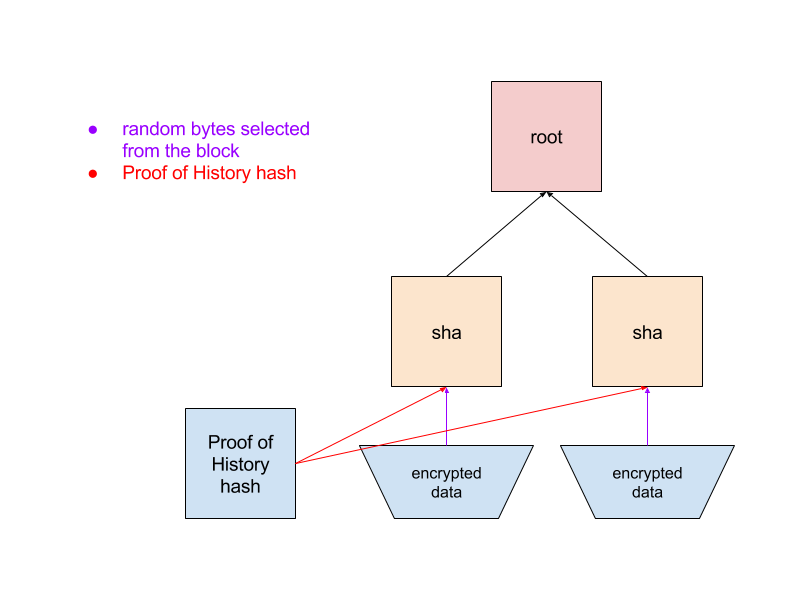
\includegraphics[width=0.6\textwidth]{figures/fig_8.png}
    \caption[Fig 8]{Fast Proof of Replication\label{fig_8}}
  \end{center}
  \end{figure}

The root is published, along with the key, and the selected hash that was generated.  The replication node is required to publish another proof in N hashes as they are generated by Proof of History generator, where N is approximately ½ the time it takes to encrypt the data.  The Proof of History generator will publish specific hashes for Proof of Replication at a predefined periods.  The replicator node must select the next published hash for generating the proof.  Again, the hash is signed, and random slices are selected from the blocks to create the merkle root.

After a period of N proofs, the data is re-encrypted with a new key.
\subsection{Verification}

With N cores, each core can stream encryption for each identity.  Total space required is 2 blocks * N cores, since the previous encrypted block is necessary to generate the next one. Each core can then be used to generate all the proofs that derived from the current encrypted block.

Total time to verify proofs is equal to the time it takes to encrypt.  The number of replication identities that can be verified at the same time is equal to the number of available cores.  Modern GPUs have 3500+ cores available to them, albeit at ½-1/3rd the clock speed of a CPU.

\subsection{Key Rotation}

Without key rotation the same encrypted replication can generate cheap proofs for multiple Proof of History sequences.  Keys are rotated periodically and each replication is re-encrypted with a new key that is tied to a unique Proof of History sequence.

Rotation needs to be slow enough that it’s practical to verify replication proofs on GPU hardware, which is slower per core than CPUs.

\subsection{Hash Selection}

Proof of History generator publishes a hash to be used by the entire network for encrypting Proofs of Replication, and for using as the pseudorandom number generator for byte selection in fast proofs.

Hash is published at a periodic counter that is roughly equal to ½ the time it takes to encrypt the data set.  Each replication identity must use the same hash, and use the signed result of the hash as the seed for byte selection, or the encryption key.

A malicious generator could inject data into the sequence prior to this hash to generate a specific hash.  Since every identity is using the same hash, a malicious generator could only benefit a single identity, as output of each signature signed with a unique private key using a cryptographic algorithm that is collision resistant.

\subsection{Proof Validation}
The Proof of History node doesn’t validate the submitted Proof of Replication proofs.  It only keep track of number of pending and verified proofs submitted by an identity.  A proof becomes verified when the replicator is able to sign the proof by 2/3rds of the validators in the network.  

The verifications are collected by the replicator via p2p gossip network, and submitted as one packet that contains 2/3rds of the validators in the network.  This packet verifies all the proofs prior to a specific hash generated by the Proof of History sequence, and can contain multiple replicator identities at once.
\subsection{Attacks}
\subsubsection{Spam}
A malicious user could create many replicator identities and spam the network with bad proofs.  To facilitate faster verification, nodes are required to provide the encrypted data and the entire merkle tree to the rest of the network when they request verification.

The Proof of Replication that is designed in this paper allows for cheap verification of any additional proofs, as they take no additional space.  But each identity would consume 1 core of encryption time.  The replication target should be set to a maximum size of readily available cores.  Modern GPUs ship with 3500 cores.

\subsubsection{Partial Erasure}

A replicator node could attempt to partially erase some of the data to avoid storing the entire state.  The number of proofs, and the randomness of the seed should make this attack difficult.

\subsubsection{Collusion with PoH generator}

A replicator identity that is colluding with the proof of history generator could inject a specific transaction at the end of the sequence before the predefined hash for random byte selection is generated.  With enough cores, an attacker could generate a hash that is preferable to the replicator identity.

This attack could only benefit a single replicator identity.  Since all the identities have to use the same exact hash that is cryptographically signed with ECCDSA (or equivalent), the resulting signature is unique for each replicator identity, and collision resistant.  A single replicator identity would only have marginal gains.
\subsubsection{Denial of Service}
The cost of adding an additional replicator identity is equal to the cost of storage.  The cost of adding extra computational capacity to verify all the replicator identities is equal to the cost of a CPU or GPU core per replication identity.

This creates an opportunity for a denial of service attack on the network by creating a large number of valid replicator identities.

To limit this attack, the consensus protocol chosen for the network can select a replication target, and award the replication proofs that meet the desired characteristics, like availability on the network, bandwidth, geolocation etc...
\section{System Architecture}

\begin{figure}
  \begin{center}
    \centering
    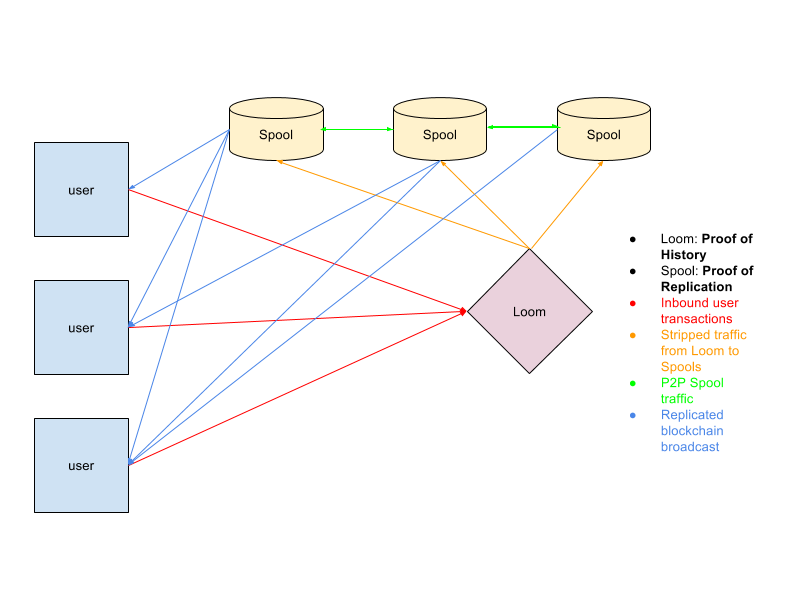
\includegraphics[width=0.6\textwidth]{figures/fig_9.png}
    \caption[Fig 9]{System Architecture \label{fig_9}}
  \end{center}
  \end{figure}

\subsection{Components}

\subsubsection{Loom, Proof of History generator}
The Loom is an elected Proof of History generator.  It consumes arbitrary user transactions and outputs a Proof of History sequence of all the transactions that guarantees a unique global order in the system.  After each batch of transactions the Loom outputs the merkle of the state that is the result of running the transactions in that order.  This merkle, and the last transactions hash is signed signed with the identity of the Loom.

\subsubsection{State}

A naive hash table addressed by the user’s address.  Each cell contains the full users address and the memory required for this computation.  For example, transactions contain
[<20 byte ripemd-160(sha256(users public key))><8 byte account value><4 byte unused>]

For a total of 32 bytes.   Proof of Stake bond’s table contains
[<20 byte ripemd-160(sha256(users public key))><64 bits bond value><Last cast vote 8 bytes><20 byte, list of uncast votes><20 bytes unused>]
For a total of 64 bytes.

\subsubsection{Spool, State Replication}
These nodes replicate the blockchain state and provide high availability of the blockchain state. The replication target is selected by the consensus algorithm, and the validators in the consensus algorithm select and vote the Proof of Replication nodes they approve of based on of-chain defined criteria.

The network could be configured with a minimum Proof of Stake bond size, and a requirement for a single replicator identity per bond.
\subsubsection{Validators}
These nodes are consuming bandwidth from Spools.  They are virtual nodes, and can run on the same machines as the Spools or the Loom, or on separate machines that are specific to the consensus algorithm configured for this network.

\subsection{Network Limits}

\begin{figure}
  \begin{center}
    \centering
    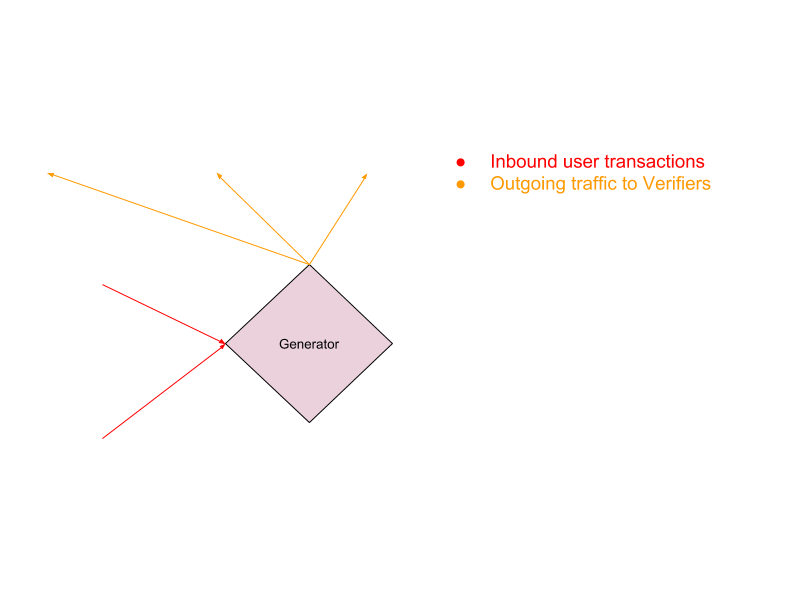
\includegraphics[width=0.6\textwidth]{figures/fig_10.png}
    \caption[Fig 10]{Loom network limits\label{fig_10}}
  \end{center}
  \end{figure}

Loom takes incoming user packets, orders them the most efficient way possible, and sequences them into a Proof of History sequence that is published to downstream Spools.  Efficiency is based on memory access patterns of the transactions, so the transactions are ordered to minimize faults and to maximize prefetching.
Incoming packet format:
[<last valid hash, 20 bytes, 8 byte counter>, <unused, 6 bits>, <payload size, 10 bits>, <payload>, <fee, 8 bytes> <from, 32 bytes>, <signature, 32 bytes>]
Size 20 + 8 + 16 + 8 + 32 + 32 = 116 bytes.  The minimal payload that can be supported would be 1 destination account
Payload: 
[<to 20 byte ripemd-160 hash>, <amount 4 byte>]
Minimum size: 24 bytes
The Proof of History sequence adds an additional hash and counter to the output: 
[<current hash, 20 byte>, <8 byte counter>, <last valid hash, 20 bytes, 8 byte counter>, <unused, 6 bits>, <size, 10 bits>, <payload>, <fee, 8 bytes> <from, 32 bytes>, <signature, 32 bytes>]
Minimum size of the output packet is: 116 + 24 + 28 = 168
Multiple transactions could be batched on the same hash.  On a 1gbps network connection the maximum number of transactions possible is 1 gigabit per second / 168 bytes = 744k tps max.  Some loss (1-4%) is expected due to ethernet framing.  The spare capacity over the target amount for the network can be used to increase availability by coding the output with Reed-Solomon codes and striping it to the available downstream Spools.
\subsubsection{Computational Limits}
Each transaction requires a digest verification.  This operation doesn’t use any memory outside of the transaction message itself, and can be parallelized independent of all the other transactions.  Thus throughput is going to be limited by the number of cores available on the system.

GPU based ECDSA verification servers have had experimental results of 900k operations per second.  (http://ieeexplore.ieee.org/document/7555336/).  This is inline with our estimate based on single NVidia 1080ti GPU. 
Memory Limits
A naive implementation of the state as a 50% full hashtable with 32 byte entries for each account, would provide 16 billion accounts.  Steady state random access to this table is measured at 1.1 * 10^7 writes or reads per second.  Based on 2 reads and two writes per transaction, memory throughput can handle 2.75m transactions per second.  This was measured on AWS 1tb x1.16xlarge instance.

\subsection{High Performance Smart Contracts}

Smart contracts are a generalized form of transactions.  These are programs that run on each node and modify the state.  This design takes advantage of extended Berkeley Packet Filter bytecode as fast and easy to analyze and JIT bytecode as the smart contracts language.

One of its main advantages is a zero cost Foreign Function Interface. This design exposes high performance intrinsics to the platform that executables can call.  Calling the intrinsics suspends that program and schedules the intrinsic on a high performance server.  Intrinsics are batched together to execute in parallel on the GPU.

\begin{figure}
  \begin{center}
    \centering
    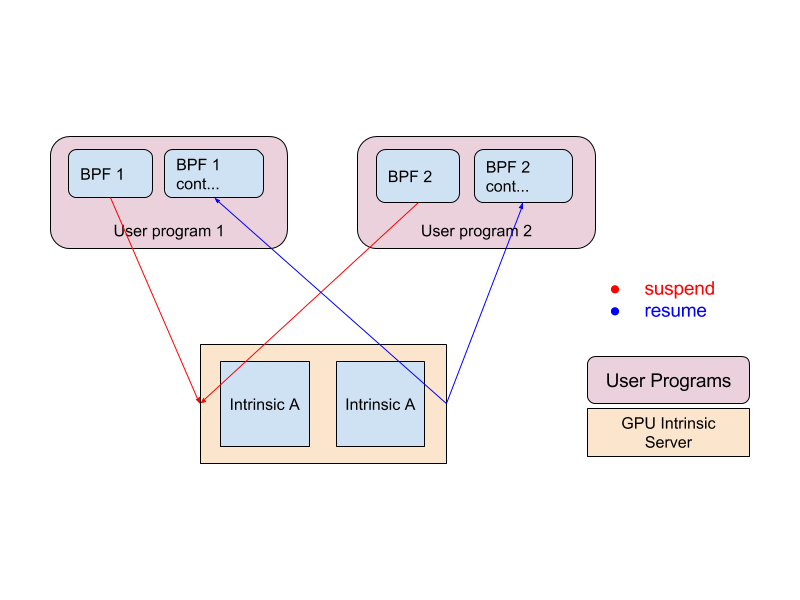
\includegraphics[width=0.6\textwidth]{figures/fig_11.png}
    \caption[Fig 11]{Executing user supplied BPF programs.\label{fig_11}}
  \end{center}
  \end{figure}

In the above example, two different user programs call the same intrinsic.  Each program is suspended until the batch execution of the intrinsics is complete.  An example common intrinsic is ECDSA verification.  Batching these calls to execute on the GPU can increase throughput by thousands of times.

This trampoline requires no native Operating System thread context switches, since the BPF bytecode has a well defined context for all the memory that is using.

eBPF backend has been included in LLVM since 2015, so any LLVM frontend language can be used to write smart contracts.  It’s been in the linux kernel since 2015, and the first iterations of the bytecode have been around since 1992.  A single pass can check eBPF for correctness, ascertain its runtime and memory requirements and convert it to x86 instructions.

\bibliographystyle{abbrv}
\bibliography{simple}

\begin{thebibliography}{9}
\bibitem{spanner}
Liskov, Practical use of Clocks
\\\texttt{ http://www.dainf.cefetpr.br/~tacla/SDII/PracticalUseOfClocks.pdf}

\bibitem{spanner}
Google Spanner TrueTime consistency
\\\texttt{ https://cloud.google.com/spanner/docs/true-time-external-consistency}

\bibitem{ordering}
Solving Agreement with Ordering Oracles
\\\texttt{ http://www.inf.usi.ch/faculty/pedone/Paper/2002/2002EDCCb.pdf}

\bibitem{tendermint}
Tendermint: Consensus without Mining
\\\texttt{https://tendermint.com/static/docs/tendermint.pdf}

\bibitem{filecoinporep}
Filecoin, proof of replication,
\\\texttt{https://filecoin.io/proof-of-replication.pdf}

\bibitem{slasher}
Slasher, A punative Proof of Stake algorithm
\\\texttt{https://blog.ethereum.org/2014/01/15/slasher-a-punitive-proof-of-stake-algorithm/}

\bibitem{delegatedpos}
BitShares Delegated Proof of Stake
\\\texttt{https://github.com/BitShares/bitshares/wiki/Delegated-Proof-of-Stake}
\end{thebibliography}

\end{document}
This is never printed
